\documentclass [MAS] {uclathes}

%%%%%%%%%%%%%%%%%%%%%%%%%%%%%%%%%%%%%%%%%%%%%%%%%%%%%%%%%%%%%%%%%%%%%%%%
%                                                                      %
%                          PRELIMINARY PAGES                           %
%                                                                      %
%%%%%%%%%%%%%%%%%%%%%%%%%%%%%%%%%%%%%%%%%%%%%%%%%%%%%%%%%%%%%%%%%%%%%%%%

\title          {Enhancing MRI-Based Alzheimer's Diagnosis: \\
                 Leveraging Synthetic Data from Generative Models to \\
                 Improve Image Classification Performance}
\author         {Daniel Kwon}
\department     {Statistics}
\degreeyear     {2024}

%%%%%%%%%%%%%%%%%%%%%%%%%%%%%%%%%%%%%%%%%%%%%%%%%%%%%%%%%%%%%%%%%%%%%%%%

\chair          {Ying Nian Wu}
\member         {Frederic Paik Schoenberg}
\member         {Nicolas Christou}

%%%%%%%%%%%%%%%%%%%%%%%%%%%%%%%%%%%%%%%%%%%%%%%%%%%%%%%%%%%%%%%%%%%%%%%%

\dedication     {\textsl{To my wife, Priya \ldots \\
                Whose unwavering patience, love, \\
                and support made this all possible}}

%%%%%%%%%%%%%%%%%%%%%%%%%%%%%%%%%%%%%%%%%%%%%%%%%%%%%%%%%%%%%%%%%%%%%%%%

\abstract{
    The advancement of generative models have enabled the creation of high-quality synthetic images, offering a 
    cost-effective solution to augment datasets in resource-intensive fields like medical imaging. This study evaluates 
    the efficacy of synthetic image augmentation for Alzheimer's disease classification using MRI data. By training 
    convolutional neural networks (CNNs) and vision transformers (ViTs) on varying proportions of original and synthetic 
    images, we assessed the impact of selective augmentation across dementia severity classes, comparing its performance 
    to traditional and automated augmentation methods

    Overall, synthetic image augmentation demonstrates significant potential, particularly for CNNs, as a complementary 
    or standalone augmentation strategy. Selectively augmenting specific classes, such as mildly and moderately demented
    cases, improved CNN performance, reducing cross-entropy loss when compared to training on the original dataset 
    alone. Synthetic augmentation often outperformed traditional augmentation, including automated methods like 
    AutoAugment. For ViTs, performance gains were minimal, reflecting the architecture's reliance on larger datasets. 
    These findings highlight its value in resource-constrained settings, emphasizing selective application to maximize 
    diagnostic accuracy in medical imaging.
}

%%%%%%%%%%%%%%%%%%%%%%%%%%%%%%%%%%%%%%%%%%%%%%%%%%%%%%%%%%%%%%%%%%%%%%%%

\usepackage{subcaption} 
\usepackage{graphicx}
\usepackage{amsmath}
\usepackage{amsfonts}
\usepackage{array, makecell}
\usepackage{multirow}
\usepackage{multicol}
\usepackage{float}
\usepackage{wrapfig,lipsum}
\renewcommand\cellset{\renewcommand\arraystretch{0.8}%
\setlength\extrarowheight{0pt}}

%%%%%%%%%%%%%%%%%%%%%%%%%%%%%%%%%%%%%%%%%%%%%%%%%%%%%%%%%%%%%%%%%%%%%%%%

\begin{document}

\makeintropages

%%%%%%%%%%%%%%%%%%%%%%%%%%%%%%%%%%%%%%%%%%%%%%%%%%%%%%%%%%%%%%%%%%%%%%%%

\chapter{Introduction}
The rapid advancements in state-of-the-art generative models have significantly simplified the production of 
high-quality synthetic images, often requiring only basic text or image prompts. Models like DALL-E can now generate 
images with a level of quality that closely approximates real images, narrowing the distinction between synthetic and 
authentic data. As the effort required to create synthetic images diminishes and their quality continues to improve, the 
potential for leveraging these images to augment datasets becomes increasingly promising—particularly in fields where 
data collection is constrained by high costs or limited resources \cite{medical_imaging}.

In the field of medical imaging, where image datasets often require specialized equipment and subject matter experts to 
capture and label images, gathering enough data to sufficiently train a classification model can be both expensive and 
time-consuming. For example, with the average cost of magnetic resonance imaging (MRI) at \$1,325 in the United States, 
a dataset consisting of a few hundred images can exceed \$1 million; image classification models often require thousands
of photos \cite{mri_cost}. 

One way computer vision models have historically attempted to remedy insufficient training datasets has been to employ 
traditional image augmentation techniques, which involve applying transformations such as flipping or blurring an 
original image to produce additional images for training. However, such transformations must be applied carefully in 
order to not lose the fidelity needed to make accurate diagnostic prediction. Transformations that alter the nature of 
the images can potentially lead to a degradation in model performance.

Augmenting image datasets with high quality synthetic images may allow for significant cost-saving while maintaining 
model performance, and previous research has found that synthetic images may play a complimentary role to image 
augmentation \cite{synthetic_imaging}. The goal of this paper is to train image classification models on a MRI dataset 
to identify the presence of varying levels of dementia and investigate the effect of different image augmentation 
policies on model performance as well as compare their performance against an augmentation policy that generates 
synthetic images.

\chapter{Dataset}

\section{Alzheimer MRI Preprocessed Dataset}
For the purposes of this paper, we use publicly available MRI images of patients with varying levels of dementia, 
labeled as \textit{not demented}, \textit{very mildly demented}, \textit{mildly demented}, and \textit{moderately 
demented}.

\begin{figure}[H]
    \centering
    \subfloat[Not \\ Demented]{
        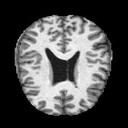
\includegraphics[width=0.225\textwidth]{figures/not-demented-example.png}}
    \hfill
    \subfloat[Very Mildly \\ Demented]{
        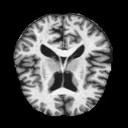
\includegraphics[width=0.225\textwidth]{figures/very-mild-demented-example.png}}
    \hfill
    \subfloat[Mildly \\ Demented]{
        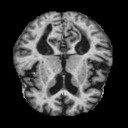
\includegraphics[width=0.225\textwidth]{figures/mild-demented-example.png}}
    \hfill
    \subfloat[Moderately \\ Demented]{
        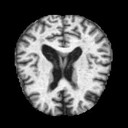
\includegraphics[width=0.225\textwidth]{figures/moderate-demented-example.png}}
    \caption{Examples of real MRI images}
\end{figure}

\begin{table}[H]
    \centering
    \begin{tabular}{|>{\centering\arraybackslash}p{0.2\linewidth}|>{\centering\arraybackslash}p{0.2\linewidth}|>{\centering\arraybackslash}p{0.2\linewidth}|>{\centering\arraybackslash}p{0.2\linewidth}|} \hline 
        Not Demented & Very Mildly Demented & Mildly Demented & Moderately Demented\\ \hline 
        2566 & 1781 & 724 & 49\\ \hline
    \end{tabular}
    \caption{Count of each class in training data}
\end{table}

These images were downloaded via the datasets module provided and maintained by Hugging Face. All images are 
in black and white and have been pre-processed to 128x128 resolution or 256x256 resolution, depending on the model being
tested \cite{alzheimer_mri_dataset}.

\section{Synthetic Images}
This paper utilizes OpenAI's Dall-E-2 to produce synthetic images. To generate synthetic images, an original image is 
supplied as a source and the generative models are prompted to creating a similar image.

In order to generate images using Dall-E-2 we utilize OpenAI's image variation API endpoint, which returns a variation 
of a given image \cite{openai_api}. 

\begin{figure}[H]
    \centering
    \subfloat[Real Image]{
        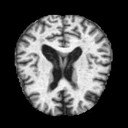
\includegraphics[width=0.25\textwidth]{figures/ModerateDemented_9.png}}
    \hspace{0.1\textwidth}
    \subfloat[Synthetic Image]{
        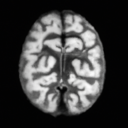
\includegraphics[width=0.25\textwidth]{figures/ModerateDemented_9_generated30.png}}
    \caption{Results of Dall-E-2's image variation generation}
\end{figure}

Dall-E-2 reliably generates images that are similar to the real MRIs that are provided. Given that dementia is often 
physically tied to brain atrophy in certain areas, the synthetic images produced by Dall-E-2 generally reproduce the 
ridges, folds, and cavities of the source images as well \cite{brain_atrophy}.

\chapter{Exploration using Grad-CAM}

In order to better understand what parts of an image classification models deem to be more "important" in regards to 
predicting the presence of dementia, we employ Gradient-weighted Class Activation Mapping, or Grad-CAM, as a way to 
represent what a convolutional neural network "sees" when classifying both real and synthetic images. Grad-CAM is a 
technique that maps the gradients of a final convolutional layer in regards to a specific class prediction to product a 
heat map. The result is a visually intuitive way of illustrating which portions of an image contribute most to a given 
classification \cite{gradcam}.

\section{Overview of Grad-CAM}

\begin{enumerate}
    \item First, calculate the gradients of the model’s output in the final convolutional layer, with respect to the 
    feature maps. Assuming \(y_{c}\) is the score for class \(c\) (before softmax) and \(\delta A^{k}\) is the feature 
    map activation of the \(k\)th layer, compute \(\frac{\delta y_{c}}{\delta A^{k}}\). 
    
    \item Next, calculate the global average pooling of the feature map. Global average pooling is a pooling operation 
    designed to generate one feature map for each corresponding category of the classification task in the last 
    convolutional layer and then take the average of each feature map \cite{networkinnetwork}.
    
    \[\alpha_{k}^{c} = \frac{1}{Z}\sum_{i}\sum_{j}\frac{\delta y_{c}}{\delta A_{ij}^{k}}\]

    \(Z\) here represents spatial dimensions of the feature map---in this case, its height and width. By dividing by 
    \(Z\), we obtain the average of gradients over all spatial locations. \(\frac{\delta y_{c}}{\delta A_{ij}^{k}}\) is 
    the gradient for class c with respect to the activation at \(A_{ij}^{k}\), or spatial location (i,j) on activation 
    layer \(k\).
    
    \item Lastly, we take the resulting importance weights in \(a_{k}^{c}\) and combine them with \(A^{k}\) to calculate 
    a weighted combination of all forward activation maps. We then apply the ReLU activation function to the resulting 
    combination in order to take the positive values only. This ensures that we are only looking parts of the image that 
    are positively correlated with a given class.

    \[L_{Grad-CAM}^{c} = ReLU(\sum_{k}\alpha_{k}^{c}A^{k})\]

    Notice that \(L_{Grad-CAM}^{c}\) will have the dimensions of the final convolutional layer and therefore is likely 
    to be smaller than the original input image. In that case, we simply upsample the result to the dimensions of our 
    original image in order to overlay the two.
\end{enumerate}

\section{Exploratory Results}

In order to better understand what our models "look at" when evaluating an image and predicting a class, we take a basic 
CNN with the same architecture outlined in chapter 5, section 1 and train it on real MRI images. While the model 
architecture is relatively simple compared to deeper networks, it is sufficient in order to explore what parts of an 
image a typical CNN focuses on. For the purposes of this exploratory analysis we only look at MRIs labeled as moderately 
demented or non-demented, as these classes are the at the most extreme ends of the spectrum and will illustrate what 
characteristics contribute to the model detecting the presence of absence dementia.

\subsection{Real vs synthetic images labeled as having moderate dementia}

\begin{figure}[H]
    \centering
    \subfloat[Real]{
        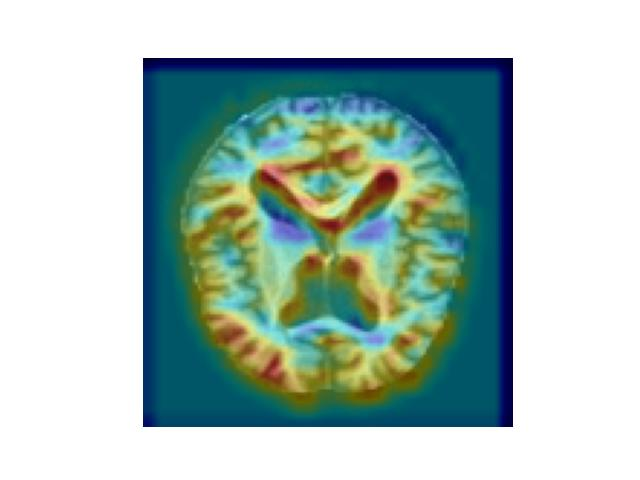
\includegraphics[width=0.45\textwidth]{figures/gradcam_images/ModerateDementedRealGradcam_predictModerateDemented.jpg}}
    \hspace{0.001\textwidth}
    \subfloat[Synthetic]{
        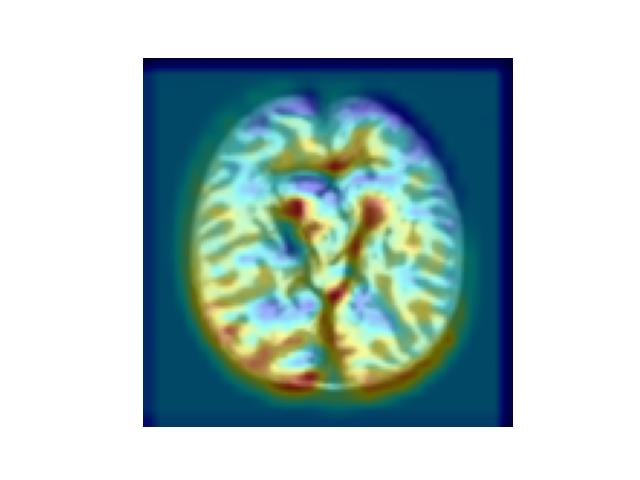
\includegraphics[width=0.45\textwidth]{figures/gradcam_images/ModerateDementedSyntheticGradcam_predictModerateDemented.jpg}}
    \caption{Grad-CAM when predicting ModerateDemented for ModerateDemented class}
\end{figure}

When looking at a real image of a brain with moderate dementia, we can see that signs of atrophy contribute to the 
likelihood that the model classifies this brain as one with moderate dementia. When applying Grad-CAM on a synthetic 
image generated via the previous original image as a source, we can see that the qualities that indicate the presence of 
dementia are also present in the synthetic images as well. While not as pronounced, the areas of atrophy in the 
synthetic brain image are present and our model focuses on those areas in both real and synthetic images.

\begin{figure}[H]
    \centering
    \subfloat[Real]{
        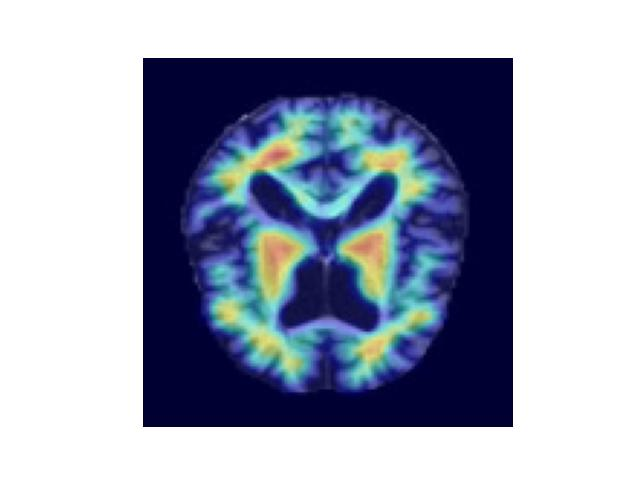
\includegraphics[width=0.45\textwidth]{figures/gradcam_images/ModerateDementedRealGradcam_predictNonDemented.jpg}}
    \hspace{0.001\textwidth}
    \subfloat[Synthetic]{
        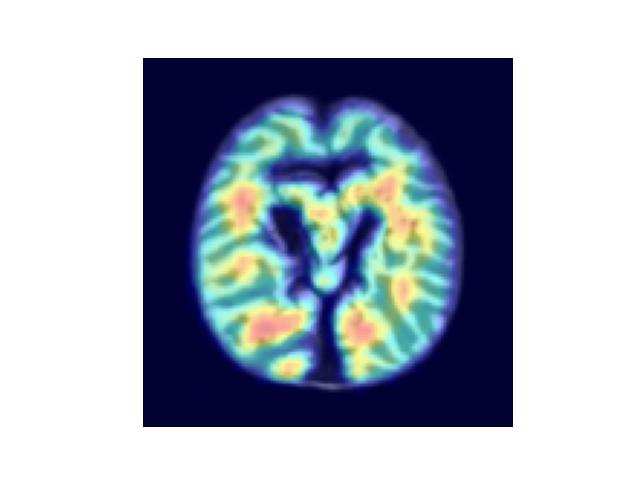
\includegraphics[width=0.45\textwidth]{figures/gradcam_images/ModerateDementedSyntheticGradcam_predictNonDemented.jpg}}
    \caption{Grad-CAM when predicting NonDemented for ModerateDemented class}
\end{figure}

The same image shows that the areas of non-atrophy, particularly those closer to the brain stem, contribute to a 
likelihood that this image would be classified as non-demented. The associated synthetic image shows similar patterns.

\subsection{Real vs synthetic images labeled as having no dementia}

\begin{figure}[H]
    \centering
    \subfloat[Real]{
        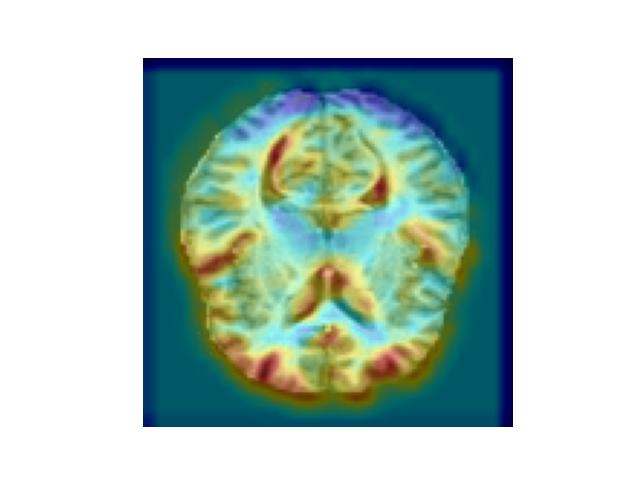
\includegraphics[width=0.45\textwidth]{figures/gradcam_images/NonDementedRealGradcam_predictModerateDemented.jpg}\label{fig:f1}}
    \hspace{0.001\textwidth}
    \subfloat[Synthetic]{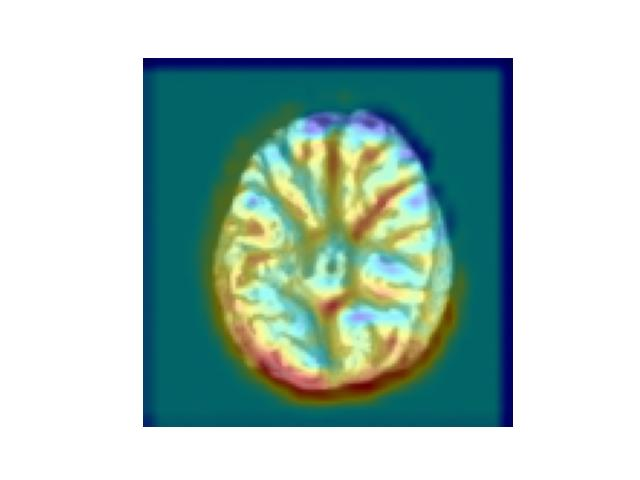
\includegraphics[width=0.45\textwidth]{figures/gradcam_images/NonDementedSyntheticGradcam_predictModerateDemented.jpg}\label{fig:f2}}
    \caption{Grad-CAM when predicting ModerateDemented for NonDemented class}
\end{figure}

When comparing real and synthetic images of a brain with no signs of dementia, we see that our synthetic image captures
the areas of non-atrophy that is present in the original source image. 

\begin{figure}[H]
    \centering
    \subfloat[Real]{
        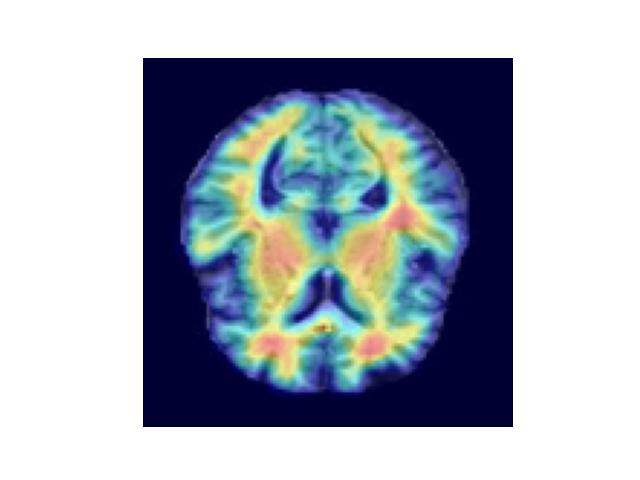
\includegraphics[width=0.45\textwidth]{figures/gradcam_images/NonDementedRealGradcam_predictNonDemented.jpg}}
    \hspace{0.001\textwidth}
    \subfloat[Synthetic]{
        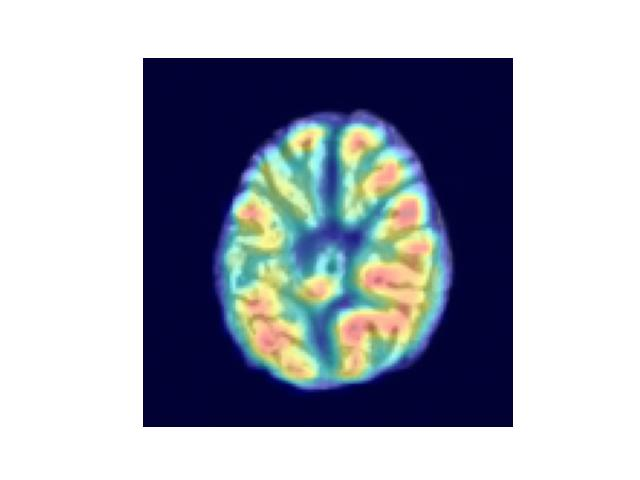
\includegraphics[width=0.45\textwidth]{figures/gradcam_images/NonDementedSyntheticGradcam_predictNonDemented.jpg}}
    \caption{Grad-CAM when predicting NonDemented for NonDemented class}
\end{figure}

There does not appear to be significant signs of atrophy present in an image of a non-demented brain---which our 
synthetic image has adequately captured. Both real and synthetic images show larger non-atrophied areas of the brain, 
which our model is focusing on as an indication of a brain without dementia.

\chapter{Background on Training Deep Learning Models}

\section{Overview of Neural Networks}
While deep learning architectures can span many layers and can incorporate many different mechanisms, at its core all 
deep learning models are neural networks. Training neural networks comprise of a few key steps. 

First, training data is input into a neural network and passed through as-is in what is known as a "forward pass." In a 
fully connected neural network, every individual neuron in a layer of the neural network is connected to each neuron in 
the preceding layer \cite{nn_intro}. 

\begin{figure}[H]
    \centering
    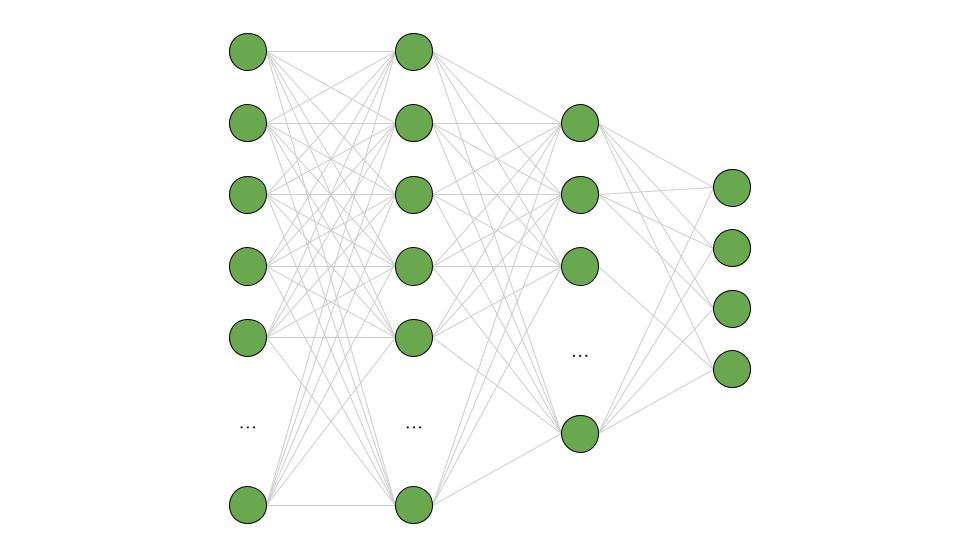
\includegraphics[width=0.75\linewidth]{figures/NN_diagram.jpg}
    \caption{An illustration of a typical fully-connected neural network}
\end{figure}

Each of these connections has a weight that stores how strong of a connection each preceding node has to the current 
node. A bias term is also present, which represents whether a neuron is general activated or not. Often, an initialized 
neural network will comprise of randomized weights and biases whereas a pre-trained model will have the weights and 
biases already defined from previous training. When training a neural network, the weights and biases are what are being 
adjusted in order to minimize loss. The formulation of a single neuron with n nodes in the previous layer is below \cite{deeplearningbook}:

\[\sigma(w_0a_0 + w_0a_0 + w_0a_0 + ... + + w_{n-1}a_{n-1} + b)\]

After the forward pass, backpropagation occurs in which the gradient (the vector of partial derivatives) of the loss 
function with respect to each weight and bias is calculated via chain rule \cite{nn_analyze}. Each gradient value 
represents the magnitude and direction of the change in our loss function given a change to that particular weight or 
bias. Because backpropagation uses the chain rule to propagate the loss backward from the output layer to the input 
layer, the process of finding the gradient of a loss function remains the same no matter how many layers are in the 
network or how many neurons are in each layer.

Once the gradient is calculated, the gradient descent algorithm is used to update the weights and biases in order to 
minimize loss. However, applying the gradient descent on an entire training dataset in a single batch is computationally 
expensive. Instead, gradient descent is often applied to subsets of the training data, called mini-batches. Each 
training iteration, or epoch, will then take a mini-batch to apply the forward and backward passes on to to updates its 
weights and biases. The result is an accurate approximation of the gradient of the loss function while significantly 
decreasing computational expenses \cite{nn_backprop}.

\section{Loss Function}
The loss function used throughout this paper when measuring model performance is cross entropy loss. Cross entropy loss 
is defined as:

\[L = -\sum_{c=1}^{C}y_{c}log(p_{c})\]

where \(C\) = the number of classes, \(y_{c}\) is the true label for class, and \(p_{c}\) is the predicted probability 
for class \(c\). Cross entropy loss therefore compares the predicted probabilities with the actual labels and penalizes 
more when the predicted probabilities for a correct class is low \cite{cross_entropy_intro}.

Cross entropy loss is better suited for measuring the performance of classification models when multiple classes are 
involved than traditional measures of error, such as the sum of residuals, as it is more sensitive to predictions that 
are "more" incorrect. In an image classification problem, a model may mislabel a given image, but the cross entropy loss 
will be lower if the predicted probability for the correct class is higher, even if the model did not ultimately end up 
labeling correctly. Contrast that with the sum of residuals, which only views predictions as completely correct or 
completely incorrect and fails distinguish between the degrees of how right or wrong a prediction can be \cite{cross_entropy_lecture}.

\begin{figure}[H]
    \centering
    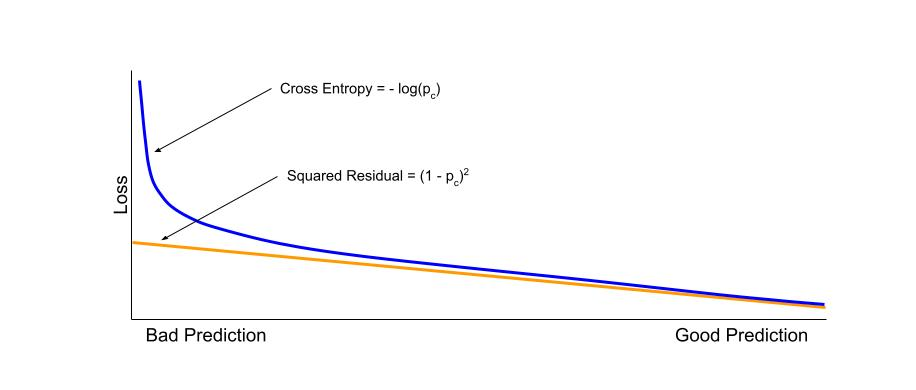
\includegraphics[width=1\linewidth]{figures/CE vs Square Residual.jpg}
    \caption{Illustration of Cross Entropy Loss vs Squared Residual \cite{cross_entropy_lecture}}
\end{figure}

Take for example, when the true label is 1 and the predicted class weight \(y_{c}\) is 0.0001---making our model 
prediction very bad. The squared residual would be \((1-0.0001)^{2} = 0.9998\) while our cross entropy loss would be 
more punitive at \(-log(0.0001) = 4\). Cross entropy loss also has a much larger gradient for very bad predictions, 
allowing our model to more quickly learn to avoid bad predictions.

\section{Gradient Descent}
As mentioned previously, performing gradient descent on every single training image can be computationally inefficient \cite{gradient_desc}. 
Instead, stochastic gradient descent which divides the training dataset into smaller batches and applied the gradient 
descent algorithm on each batch, can significantly reduce runtime. 

In addition to dividing the training dataset into mini-batches, there are other methods that make optimization via 
gradient descent more efficient---namely, learning rate and momentum.

\subsection{Learning Rate}
The formulation for stochastic gradient descent is defined as \cite{deeplearningbook}:
\[\theta_{t+1} = \theta_{t} - \eta\nabla_{\theta}L(\theta_{t};x^{(i)})\]
Where:
\begin{itemize}
    \item \(\theta_{t}\) is the model's weights and biases at iteration \(t\)
    \item \(\eta\) is the learning rate
    \item \(\nabla_{\theta}L(\theta_{t};X^{(i)})\) is the gradient of the loss function at time \(t\) with respect to 
    \(x^{(i)}\)
    \item \(x^{(i)}\) is a randomly selected mini-batch
\end{itemize}

The learning rate is a critical parameter for the training of any deep learning model and can dramatically effect how 
the gradient descent algorithm behaves. Learning rate can be understood intuitively as the step size the optimization 
algorithm takes when it decides which direction to step---too large of a learning rate can lead to sub-optimal changes 
to a network's weights and biases; too small and achieving model convergence can much longer.

Furthermore, the learning rate does not necessarily need to be constant throughout the entire optimization process. It 
can vary over time with a larger learning rate at the beginning of the training, when large steps along the gradient is 
appropriate, and reducing later in training process, when smaller learning rates are more appropriate.

\subsection{Momentum}
Momentum takes into account the gradient at previous steps, beyond simply looking at the gradient at time \(t-1\). By 
doing so, the gradient descent algorithm tends to stay in the direction where the gradient has consistently pointed 
towards. The formulation for stochastic gradient descent with momentum is defines as \cite{deeplearningbook}:
\[\theta_{t+1} = \theta_{t} - \eta v_{t}\]
Where \(v_{t}\) is known as the velocity term, defined as:
\[v_{t} = \beta v_{t-1} + (1 - \beta) \nabla_{\theta} L(\theta_{t})\]
Where:
\begin{itemize}
    \item \(\beta\) is the momentum coefficient, which determines how much of the previous gradients carry over into the 
    latest velocity calculation at time \(t\)---this parameter can be set between 0 and 1
    \item \(\nabla_{\theta} L(\theta_{t})\) is the gradient of the loss function at time \(t-1\)
\end{itemize}

\subsection{Adam Optimizer}
Adaptive Moment Estimation, also known as Adam Optimization, combines aspects of both a variable learning rate as well 
as momentum in order to develop an optimization algorithm that efficiently calculates the gradient \cite{adam}. Gradient descent 
using Adam optimization is defined as:
\[\theta_{t+1} = \theta_{t} - \frac{\eta}{\sqrt{\hat{v_t}} + \epsilon} \hat{m_{t}}\]
Where:
\begin{itemize}
    \item \(\hat{m_{t}}\) is known as the bias correction for the first moment and defined as \(\frac{m_t}{1-\beta_1^t}\)
    \item \(\hat{v_t}\) is known as the bias correction for the second momemt and defined as \(\frac{v_t}{1-\beta_2^t}\)
    \item \(m_t = \beta_1 m_{t-1} + (1 - \beta_1) \nabla_{\theta} L(\theta_t)\)
    \item \(v_t = \beta_2 v_{t-1} + (1 - \beta_2) (\nabla_{\theta} L(\theta_t))^2\)
    \item \(\beta_1\) is the decay rate for the first moment
    \item \(\beta_2\) is the decay rate for the second moment
\end{itemize}

The first moment \(m_t\) allows the Adam optimization algorithms to take into account momentum by taking the weighted 
average of past gradients. The second moment \(v_t\) acts as an adjustment to the learning rate and allows Adam 
algorithm to have a variable learning rate based on previous squared gradients. For all models trained in this paper, we 
use the Adam optimizer.

\section{Fine-tuning Pre-trained Models}
Often times, computer vision models require a large number of images as well as a significant amount of computation 
time. In order to accelerate the training process, many image classification models will utilize a pre-trained model, 
instead of starting training from randomly initialized weights and biases. A common image dataset used to pre-train 
models is the ImageNet-1000 dataset, which is comprised of 1000 distinct classes, 1,281,167 training images, 50,000 
validation images and 100,000 test images \cite{transfer}.

Once a model is pre-trained, fine-tuning can take two forms---either progressing through training as you normally would
with images intended for fine-tuning (i.e., your dataset) or freezing all weights in the pre-trained model (essentially 
locking the model from any further training) and re-training only the fully connected neural nerwork appended to the 
pre-trained model. If the latter method is used, the pre-trained model can regarded as a fixed feature extractor for an 
image. For the purposes of our paper, all pre-trained models are fine-tuned by re-training on our dataset.

\chapter{Overview of Model Architectures}
In order to gain an understanding as to how both convolution-based and attention-based architectures react to the 
introduction to synthetic data in training, We tested three different deep learning model architectures for our image 
classification models---a basic Convolutional Neural Network (CNN), a pre-trained ResNet-18 model, and a pre-trained 
Vision Transformer (ViT).

\section{Convolutional Neural Networks}

\begin{figure}[h]
    \centering
    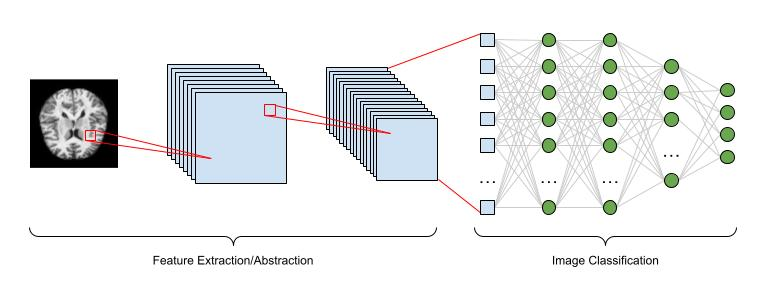
\includegraphics[width=0.9\linewidth]{figures/CNN-diagram.jpg}
    \caption{Typical CNN Architecture \cite{cnn_diagram}}
\end{figure}

CNNs are a deep learning architecture that is comprised of convolutional layers---which abstract an image to a feature 
map, pooling layers---which reduce the dimensions of data by combining the outputs of adjacent layers via downsampling, 
and fully connected layers---which are neural networks that take the final activations from the convolutional and 
pooling layers to generate class weights \cite{cnn_intro}.

Convolutional layers are a key component of convolutional neural networks and act as a way for the network to 
extract abstract features from an image. The primary operating mechanism of a convolutional layer comprises of a kernel,
or a filter that is applied to the original image.

\begin{figure}[H]
    \centering
    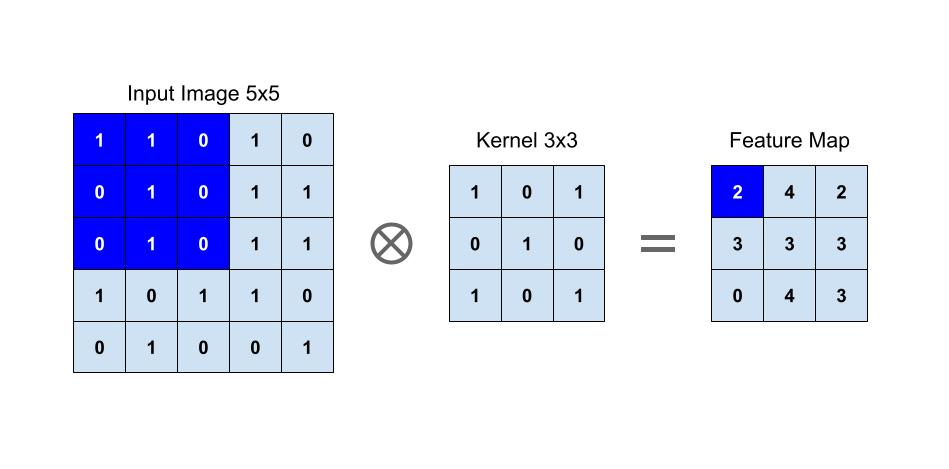
\includegraphics[width=0.6\linewidth]{figures/convolutional_layer_illustration.jpg}
    \caption{Illustration of Convolutional Layer \cite{convolution_diagram}}
\end{figure}

Often, convolutional layers may stack multiple kernels resulting in activation maps with more channels. As subsequent 
layers get deeper, more complex and increasingly abstract features are extracted from the original image. While the 
kernels from the earlier layers of a CNN may learn to identify basic shapes and patterns, kernels in deeper layers may 
learn to identify specific edges and details.

\begin{figure}[H]
    \centering
    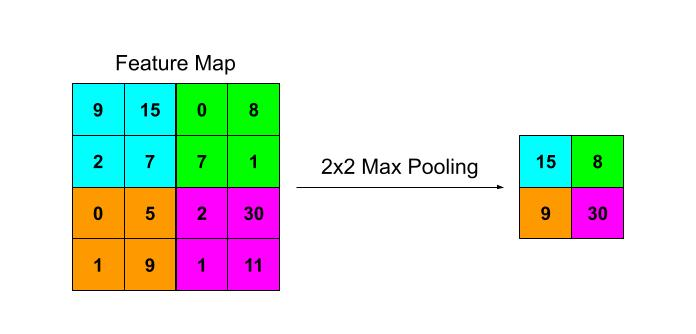
\includegraphics[width=0.55\linewidth]{figures/maxpooling_illustration.jpg}
    \caption{Illustration of 2x2 Max Pooling \cite{max}}
\end{figure}

Though not explicitly required, max pooling layers frequently follow convolutional layers. Max pooling layers 
essentially downsample the activation map so that the important features and spatial relationships contained in an image
are captured while removing unnecessary details and reducing the feature map's dimensions, thereby improving 
computational efficiency of the network.

\begin{figure}[H]
    \centering
    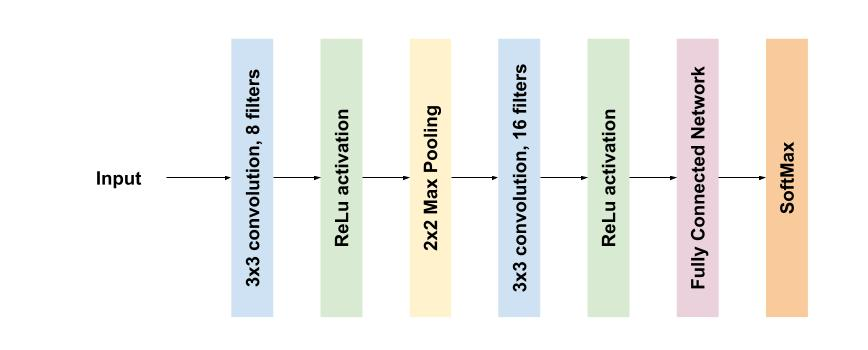
\includegraphics[width=0.8\linewidth]{figures/basic_cnn_architecture.jpg}
    \caption{Basic CNN Architecture}
\end{figure}

For the purposes of this paper, the CNN we train from scratch consists of 2 convolutional layers, each paired with a 
ReLU activation function and a max pooling layer. After all feature extraction layers are complete, the final activation 
layer is fed into a fully connected neural network with 2 hidden layers and an output layer that predicts probabilities 
weights for each of our four classes.

\section{ResNet-18}
The second model architecture we test is a ResNet-18 model, pre-trained on the ImageNet-1000 dataset. The ResNet 
architecture is similar to a basic convolutional neural network but adds two additional components---skip connections 
and residual blocks.

\begin{figure}[H]
    \centering
    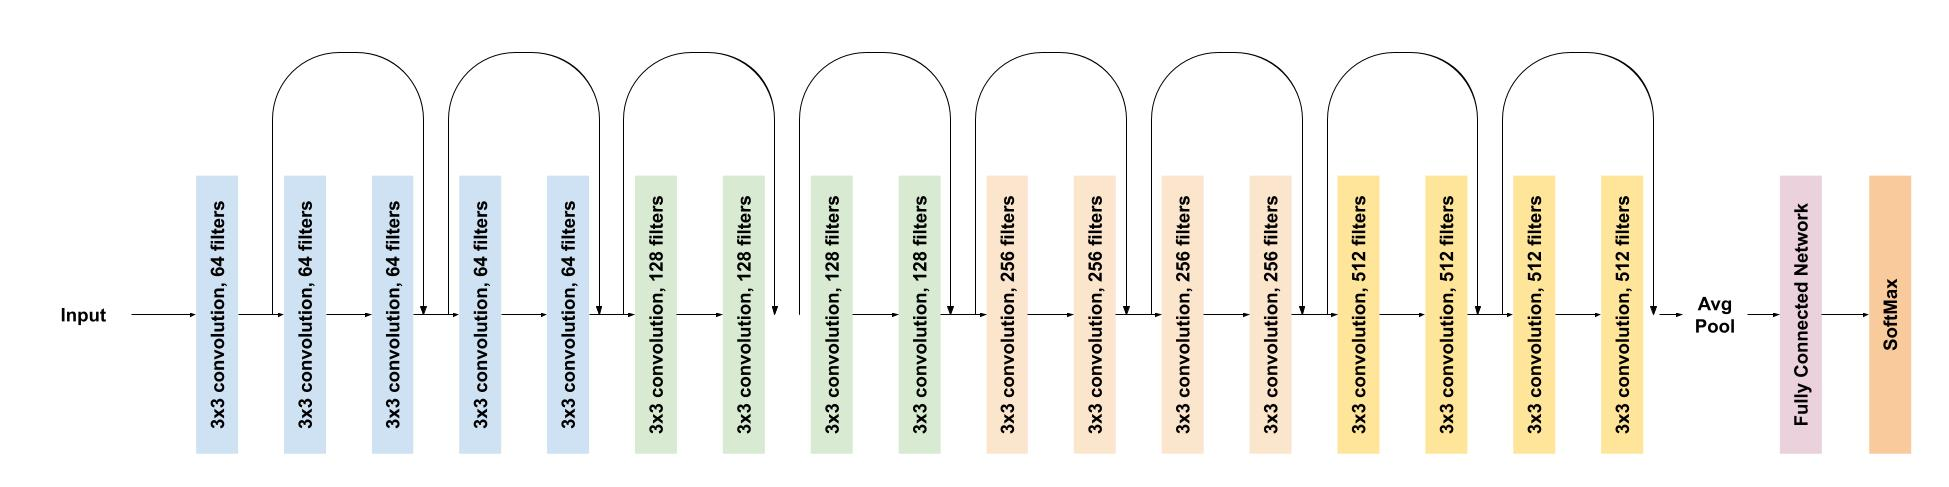
\includegraphics[width=1\linewidth]{figures/resnet18_architecture.jpg}
    \caption{ResNet-18 Architecture \cite{resnet}}
\end{figure}

Skip connections allow the network to skip a convolutional layer entirely thereby skipping training for some layers.
Doing so helps to avoid a phenomenon known as vanishing gradients---which occurs in deep networks where the gradient 
calculated via backpropagation becomes so small that weights from earlier layers become insignificant and changes to the 
input image cease to meaningfully affect feature mapping in deeper layers. Skip connections allow the ResNet model to 
build deep networks while avoiding vanishing gradients by giving the model a mechanism in which training a layer can be 
skipped entirely.

ResNet architectures are also characterized by their use of residual blocks, which consistent of 2 convolutional layers 
and a skip connection. Residual blocks allow the ResNet model to train on the residual between layers, or the difference 
between the input and the ideal output of the layers \cite{resnet}. 

\[y = F(x) + x\]

Where:
\begin{itemize}
    \item \(x\) is input fed into the residual block
    \item \(F(x)\) is output coming from the residual block
    \item \(y\) is desired final output coming from the residual block
\end{itemize}

Therefore, \(F(x) = y - x\) makes \(F(x)\) the residual of y and x. ResNets train by using residual blocks to learn the 
residual mapping, instead of being forced to train each convolutional layer and the desired feature map (although that 
is still an option left for the model to evaluate). By doing so, the ResNet remains computationally efficient while 
maintaining the ability to extract features, either through its traditional convolutional layers or via a residual 
block. 

\section{Vision Transformers}

The last type of model architecture tested---known as vision transformers or ViT for short---is one that foregoes the 
use of convolutional layers entirely and instead utilizes the attention mechanism to capture spatial relationships and 
abstract features \cite{vit}. 

\begin{figure} [H]
    \centering
    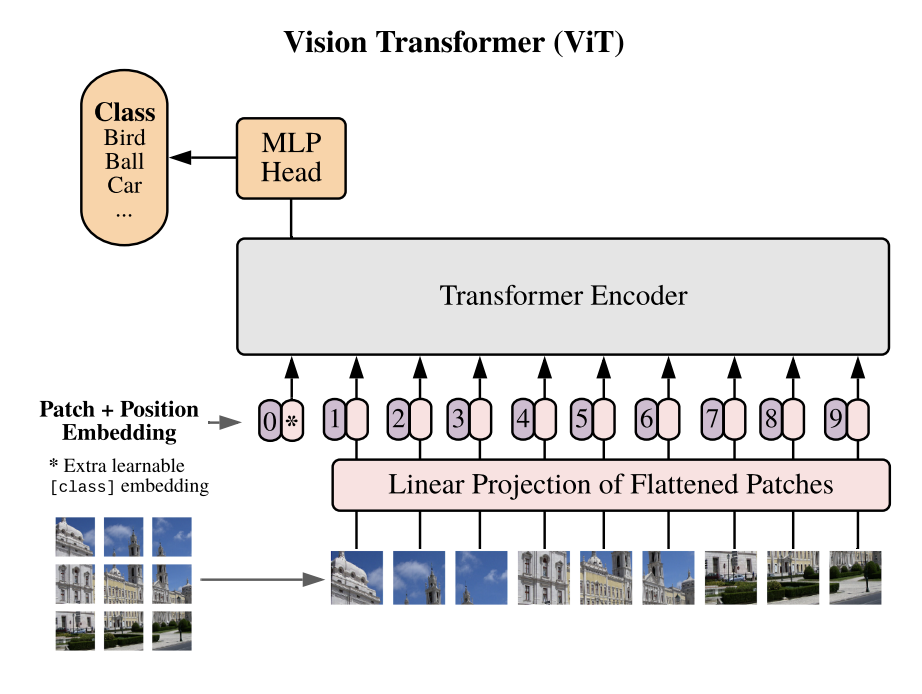
\includegraphics[width=0.6\linewidth]{figures/ViT Architecture.png}
    \caption{ViT Architecture \cite{vit}}
\end{figure}

The transformer architecture is often utilized in natural language processing tasks and serves as the 
architectural foundation for cutting edge large language models such as ChatGPT, Llama, Gemini, and Claude. 

Because applying transformers for the purpose of image classification closely parallels how they are employed for text
generation, each transformer component reviewed in this section will be accompanied with an analogous example of how the
component would work in a text transformer whenever possible.

\subsection{Background on Embeddings}
Before any data can be used as an input into a transformer, it must first be turned into a numeric representation so 
that the appropriate operations can be performed on it. For example, if an embedding has three dimensions you can 
imagine the embeddings for words such as "jump" and "leap" to have high cosine similarity, even if they are different 
words \cite{deeplearningbook}.

\begin{figure} [H]
    \centering
    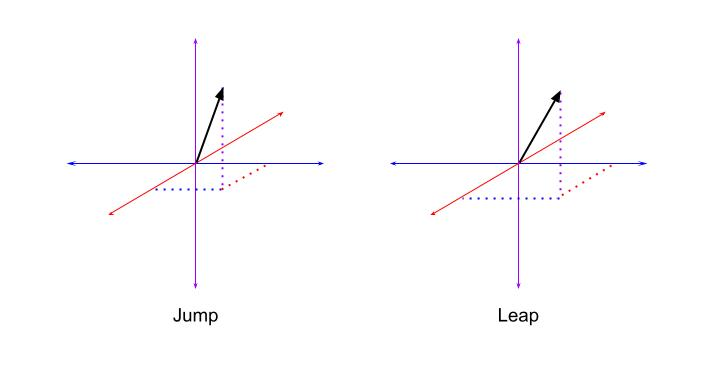
\includegraphics[width=1\linewidth]{figures/Cosine Similarity Example.jpg}
    \caption{Hypothetic 3-dimensional word embeddings}
\end{figure}

In practice, embeddings can be tens of thousands of dimensions. It is also worth noting that these embeddings are not 
static representations but trainable parameters that can be modified and adjusted as the transformer trains. 

\subsection{Patch Embeddings and Positional Encoding}
In a ViT, rather than words (or tokens) being transformed into embeddings, the image is broken up into a series of 16x16
images and flattened into a 256 dimensional vector \cite{vit}. An original image that is \(x \in \mathbb{R}^{H \times W \times C}\)
is therefore split into patches that are  \(\mathbb{R}^{P^2 \times C}\). Therefore across \(N\) patches, we have matrix
\(x_p \in \mathbb{R}^{N \times (P^2 \cdot C)}\).

Where:
\begin{itemize}
    \item \(H\) and \(W\) is the height and width of the original image
    \item \(C\) is the number of channels in the original image
    \item \(P\) is the dimension of the \(P \times P\) patch
    \item \(N = HW/P^2\) is used to calculate the needed number of patches, given a \(P \times P\) patch size
\end{itemize}


\(x_p\) is then unrolled to a vector and multiplied by an embedding matrix \(E\) to get the patch embedding. 

\[z_i = x_p \cdot E\]

Where:
\begin{itemize}
    \item \(E \in \mathbb{R}^{(P^2 \cdot C) \times D}\) is a projection matrix with learnable weights
    \item \(x_p\) is a given image patch, unrolled into vector form
\end{itemize}

The patch embedding is then combined with the positional encoding by summing it with the patch embedding in order to 
give the transformer the ability to track where each image patch is relative to the original image. The positional 
embedding represents the relative position of the original image that the image patch is sourced from. The resulting 
patch embedding and position encoding are then fed into a transformer architecture similar to how a string of token 
embeddings are fed into a traditional transformer used for natural language processing.

\subsection{Transformer Architecture}
The transformer encoder in a ViT consists of alternating layers of multi-headed self attention and MLP blocks, with 
layer normalization applied before every block and residual blocks after every block.

\begin{figure} [H]
    \centering
    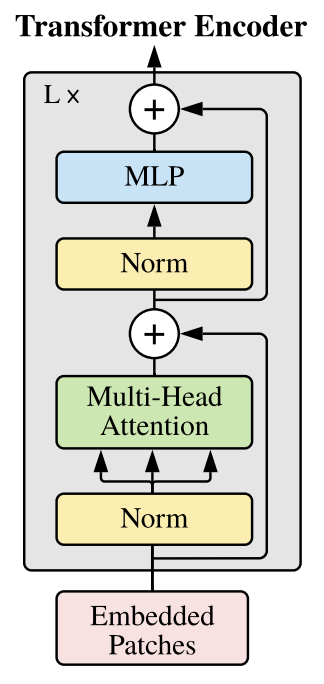
\includegraphics[width=0.2\linewidth]{figures/ViT Encoder Architecture.png}
    \caption{ViT Encoder Architecture \cite{vit}}
\end{figure}

The ViT architecture is notable for its usage of the multi-head attention block, which combine query (\(Q\)), key 
(\(K\)), and value (\(V\)) matrices in order to allow the model to "pay attention" to certain patches \cite{dot}. 

\[Attention(Q,K,V) = softmax(\frac{QK^T}{\sqrt{d_k}})V\]

Where:
\begin{itemize}
    \item \(Q\), \(K\), and \(V\) are the query, key, and value matrices, respectively
    \item \(d_k\) is the dimensions of the key vectors, such that dividing by \(\sqrt{d_k}\) ensures that the variance 
    of \(q \cdot k\) is 1
\end{itemize}

In order to pay attention to different image patches under different contexts the ViT architecture uses multi-head 
attention, which allows for multiple attention mechanisms in parallel. 

\[MultiHead(Q,K,V) = [head_1, head_2, ... , head_h]W_0\]

Where:
\begin{itemize}
    \item \(head_i = Attention(QW_i^Q, KW_i^K, VW_i^V)\)
    \item \(W\) are all learnable parameter matrices
\end{itemize}

Intuitively, multi-head attention allows the ViT model to pay attention to different parts of the image for different 
contexts. For example, certain characteristics of an image may warrant more attention when defining segment boundaries, 
while those same characteristics may not warrant attention when considering segment orientation \cite{att}.

\chapter{Overview of Image Augmentation Techniques}
In addition to different model architectures, we also test combinations of different traditional image augmentation 
policies and image augmentation via synthetic images. See below for all image augmentation pairings tested:

\begin{multicols}{2}
    \raggedcolumns
    \textbf{Image Augmentation Policies}
    \begin{itemize}
        \item Random horizontal flipping
        \item AutoAugment policy
        \item No image augmentation
    \end{itemize}
    
    \columnbreak
    
    \textbf{Synthetic Image Policies}
    \begin{itemize}
        \item Synthetic image generation via Dall-E-2
        \item No synthetic image augmentation
    \end{itemize}
\end{multicols}

\section{Rudimentary Image Augmentation}
Image augmentation in its simplest basic form is a policy that consists of basic image transformations, such as flipping
an image on its horizontal or vertical axis. Often, this image augmentation is applied randomly based on a probability 
defined prior to training. Because rudimentary image augmentation is cost effective and can result in improved 
performance for a image classification model with relatively low computational cost, it is frequently used to augment 
limited datasets are difficult or expensive to collect and/or label \cite{augment}.

\begin{figure} [H]
    \centering
    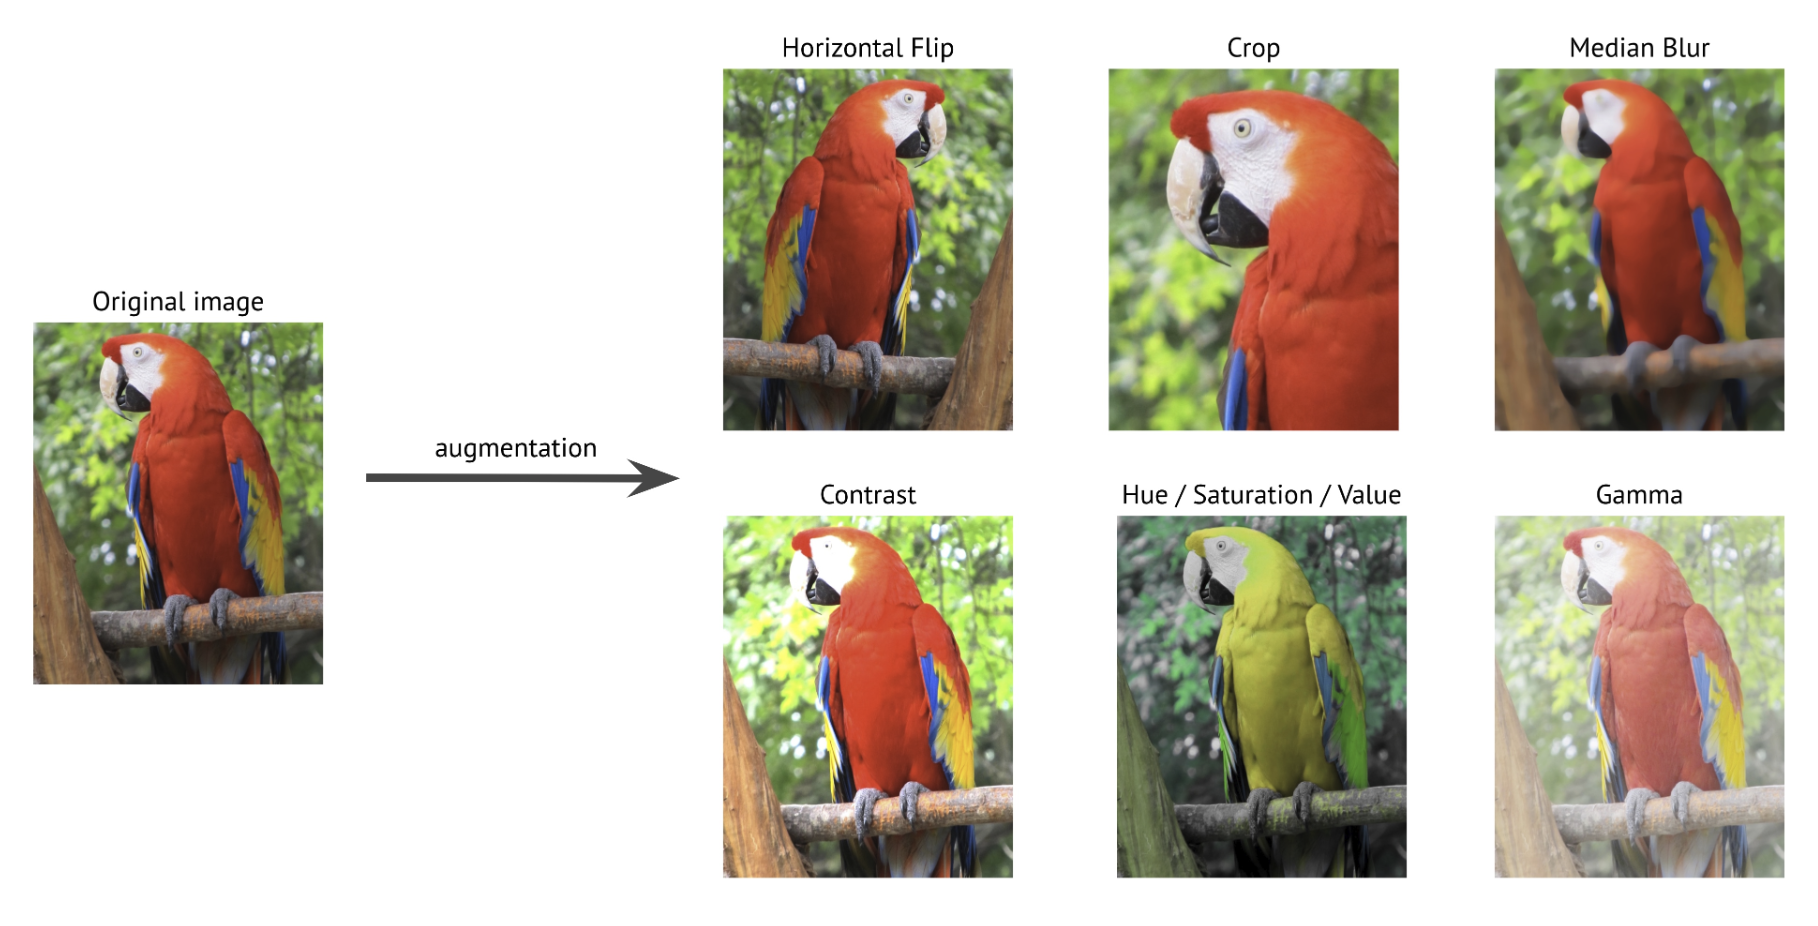
\includegraphics[width=0.75\linewidth]{figures/basic-image-augmentation-example.png}
    \caption{basic image augmentation examples \cite{augment}}
\end{figure}

For the purposes of this paper, the basic image augmentation policy applies a horizontal flip randomly with a 
probability of 50\%. Other image transformations, such as cropping or adjusting the color saturation, were not tested 
due to the nature or our training images. The MRI dataset is in grayscale and intended to capture the entirety of the 
brain and therefore cropping or changing the color of the image in any way did not fit our particular use case. 

\section{AutoAugment}
AutoAugment is an image augmentation policy that was developed by researchers at Google. It takes existing augmentation 
procedures, such as the ones listed in the previous section, and automates the selection of which procedures to include,
in order to select the optimal transformations in order to improve the model performance. The result is a systemic 
augmentation policy that eliminates the need for manual tuning \cite{autoaugment}. 

The AutoAugment policy works by employing a reinforcement learning framework in order to find optimal policies. Using a 
neural network designated as the controller, the AutoAugment policy explores a defined search space of possible 
transformations---with each transformation having a probability of being applied and a magnitude of the transformation.
The controller then tests augmentation policies within the search space in order to train a model. The model's 
subsequent performance is measured against a validation dataset and is used to further optimize the image augmentation 
policy. This feedback loop continues until controller has found an optimal augmentation policy.

AutoAugment is more computationally expensive than a basic image augmentation policy, as it involves training the 
controller neural network before it can be used in the training of the actual model itself, which can be an entirely 
separate deep learning model. To address this, AutoAugment policies can be pre-trained on larger datasets---which are 
then generalized to other images. In this paper, we tested an AutoAugment policy pre-trained on the popular and widely 
available IMAGENET dataset.

\section{Synthetic Image Generation Policy}
The proposed image augmentation policy via synthetic image generation exists as a step that exists prior to any 
traditional image augmentation steps, generating synthetic images that are passed along to the subsequent image 
transformations that exist downstream. Given a proportion of original training images to utilize for label \(i\)---
denoted as \(X_{i}\)---and the desired proportion of synthetic images to augment the training data for label \(i\)---
denoted as \(Y_{i}\)---we combine both synthetic and original images in order to create a mixed train dataset used to 
train the image classification model. In practice, \(X_{i}\) would almost always be 100\% as you generally want to train
on available data you have; however, we test different values of \(X_{i}\) in order to test the efficacy of our image 
generation policy across a range of possible dataset sizes.


\begin{figure} [H]
    \centering
    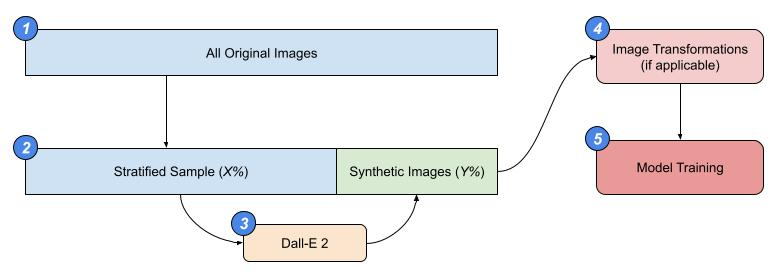
\includegraphics[width=1\linewidth]{figures/image_generation_policy.jpg}
    \caption{Illustration of the image generation policy}
\end{figure}

The figure above illustrates our image generation policy in order to generate our mixed training set (i.e., containing 
both original and synthetic images)
\begin{enumerate}
    \item First, we take a random sample of our original images
    \item The sample is sent to Dall-E 2 via OpenAI's API in order to generate an image variation
    \item Image transformations are applied to our entire mixed training set (if applicable)
    \item Mixed training set, post transformations/augmentation, is used to train the image classification model
\end{enumerate}

\chapter{Methodology and Results}

\section{Methodology}
To test the effects that synthetic images have on image classification performance, we tested a variety of model 
architectures paired with differing image augmentation protocols. We also tested protocols that involved synthetic 
image augmentation for all classes in our original dataset and ones that involve augmentation for select classes only. 
Each combination is trained 20 times on independent samples in order to get a distribution of results and reported 
results are based on the median of the distribution of measured performances.

Scenarios tested were:
\begin{itemize}
    \item Training on 100\% of available training data
    \item Training on 100\% of available training data and an additional 20\% consisting of synthetic images
    \item Training on 80\% of available training data
    \item Training on 80\% of available training data and an additional 20\% consisting of synthetic images
    images
\end{itemize}

To avoid overfitting our models, after each training epoch the performance of the model is tested against a validation 
data set that is held out. If the model fails to improve (i.e., reduce the loss function) against the validation data 
set for 2 consecutive epochs, that particular training run is ended and the model performance is logged.

\section{Basic CNN Results}

\begin{table}[htbp]
    \begin{center}
        \scriptsize{
            \renewcommand{\arraystretch}{2}
            \begin{tabular}{ |p{0.4cm}|p{5cm}|p{2.5cm}|p{2.5cm}|p{2.5cm}| }
                \hline
                \multicolumn{5}{|c|}{Cross Entropy Loss} \\
                \hline
                \multicolumn{2}{|c|}{Scenario} & \makecell{No \\ Augmentation} & \makecell{Random \\ Horizontal \\ Augment} & \makecell{AutoAugment} \\
                \hline
                \makecell{1} & \makecell{100\% Real / 0\% Synthetic} & \makecell{0.113512} & \makecell{0.173663} & \makecell{0.15266} \\
                \makecell{2} & \makecell{80\% Real / 0\% Synthetic} & \makecell{0.23912} & \makecell{0.270616} & \makecell{0.274309} \\
                \makecell{3} & \makecell{100\% Real / 20\% Synthetic \\ (Mild \& Moderate Demented Only) \\}  & \makecell{0.103296} & \makecell{0.169054} & \makecell{0.137484} \\
                \makecell{4} & \makecell{80\% Real / 20\% Synthetic \\ (Mild \& Moderate Demented Only) \\}  & \makecell{0.213611} & \makecell{0.247438} & \makecell{0.242083} \\
                \makecell{5} & \makecell{100\% Real / 20\% Synthetic \\ (All Classes) \\}  & \makecell{0.11991} & \makecell{0.167369} & \makecell{0.178442} \\
                \makecell{6} & \makecell{80\% Real / 20\% Synthetic \\ (All Classes) \\}  & \makecell{0.267219} & \makecell{0.273711} & \makecell{0.276593} \\
                \hline
            \end{tabular}}
        \quad
    \end{center}
    \caption{CNN results}
\end{table}

The basic image augmentation and AutoAugment protocols resulted in a slight degradation of model performance across all 
training scenarios, illustrating that simply applying image augmentation is not always recommended when training image 
classification models.

Similarly, synthetic image augmentation applied equally across all image classes results in a slight increase in cross 
entropy loss. This is likely due to Dall-E-2 struggling to produce non-demented images with sufficient fidelity.

However, models trained on datasets with image augmentation applied to only the 2 most demented image classes (labeled 
as mildly and moderately demented) performed better than those trained on synthetic images alone. Comparing scenarios 1 
and 3, synthetic image augmentation to specific classes resulted in a 9.0\% decrease in cross entropy loss when paired 
with the best performing traditional image augmentation protocol (no augmentation), reducing loss from from 11.4\% to 
10.3\%. This holds true for scenarios 2 and 4 as well, which trained models on 80\% of the available real training 
images. The introduction of synthetic images reduced error by 10.7\%, from 23.9\% to 21.4\%.

\section{ResNet Results}
\begin{table}[htbp]
    \begin{center}
        \scriptsize{
            \renewcommand{\arraystretch}{2}
            \begin{tabular}{ |p{0.4cm}|p{5cm}|p{2.5cm}|p{2.5cm}|p{2.5cm}| }
                \hline
                \multicolumn{5}{|c|}{Cross Entropy Loss} \\
                \hline
                \multicolumn{2}{|c|}{Scenario} & \makecell{No \\ Augmentation} & \makecell{Random \\ Horizontal \\ Augment} & \makecell{AutoAugment} \\
                \hline
                \makecell{1} & \makecell{100\% Real / 0\% Synthetic} & \makecell{0.126419} & \makecell{0.216701} & \makecell{0.954748} \\
                \makecell{2} & \makecell{80\% Real / 0\% Synthetic} & \makecell{0.209497} & \makecell{0.280073} & \makecell{0.955477} \\
                \makecell{3} & \makecell{100\% Real / 20\% Synthetic \\ (Mild \& Moderate Demented Only) \\}  & \makecell{0.119202} & \makecell{0.175533} & \makecell{0.592514} \\
                \makecell{4} & \makecell{80\% Real / 20\% Synthetic \\ (Mild \& Moderate Demented Only) \\}  & \makecell{0.194314} & \makecell{0.259539} & \makecell{0.785979} \\
                \makecell{5} & \makecell{100\% Real / 20\% Synthetic \\ (All Classes) \\}  & \makecell{0.137582} & \makecell{0.212513} & \makecell{0.934237} \\
                \makecell{6} & \makecell{80\% Real / 20\% Synthetic \\ (All Classes) \\}  & \makecell{0.182547} & \makecell{0.284151} & \makecell{0.989995} \\
                \hline
            \end{tabular}}
        \quad
    \end{center}
    \caption{ResNet results}
\end{table}

ResNet models reacted to synthetic images similarly to our basic CNN architecture, with findings from the ResNet model 
training scenarios aligning directionally with the results found when using the CNN architecture. Comparing scenarios 1 
and 3, synthetic image augmentation to specific classes resulted in a 5.7\% decrease in cross entropy loss when paired 
with the best performing traditional image augmentation protocol (no augmentation), reducing loss from from 12.6\% to 
11.9\%. The same is true for scenarios 2 and 4 with synthetic images reducing error by 7.2\%, from 20.9\% to 19.4\%.

\section{ViT Results}
\begin{table}[htbp]
    \begin{center}
        \scriptsize{
            \renewcommand{\arraystretch}{2}%
            \begin{tabular}{ |p{0.4cm}|p{5cm}|p{2.5cm}|p{2.5cm}|p{2.5cm}| }
                \hline
                \multicolumn{5}{|c|}{Cross Entropy Loss} \\
                \hline
                \multicolumn{2}{|c|}{Scenario} & \makecell{No \\ Augmentation} & \makecell{Random \\ Horizontal \\ Augment} & \makecell{AutoAugment} \\
                \hline
                \makecell{1} & \makecell{100\% Real / 0\% Synthetic} & \makecell{1.027283} & \makecell{1.035484} & \makecell{1.039906} \\
                \makecell{2} & \makecell{80\% Real / 0\% Synthetic} & \makecell{1.037404} & \makecell{1.038775} & \makecell{1.040221} \\
                \makecell{3} & \makecell{100\% Real / 20\% Synthetic \\ (Mild \& Moderate Demented Only) \\}  & \makecell{1.030077} & \makecell{1.03741} & \makecell{1.042706} \\
                \makecell{4} & \makecell{80\% Real / 20\% Synthetic \\ (Mild \& Moderate Demented Only) \\}  & \makecell{1.035646} & \makecell{1.056816} & \makecell{1.05099} \\
                \makecell{5} & \makecell{100\% Real / 20\% Synthetic \\ (All Classes) \\}  & \makecell{1.037403} & \makecell{1.035373} & \makecell{1.039411} \\
                \makecell{6} & \makecell{80\% Real / 20\% Synthetic \\ (All Classes) \\}  & \makecell{1.041386} & \makecell{1.034649} & \makecell{1.039104} \\
                \hline
            \end{tabular}}
        \quad
    \end{center}
    \caption{ViT results}
\end{table}

ViT models consistently underperformed compared to CNNs, regardless of the augmentation protocols applied during 
training. Among the tested configurations, ViT models achieved their best performance when trained on the full training 
dataset without traditional or synthetic image augmentation, suggesting a limited benefit from synthetic augmentation in 
comparison to CNN architectures.

However, when comparing scenarios involving combinations of traditional and synthetic augmentation (e.g., scenarios 1 
and 5, as well as 2 and 6), there was a slight improvement in performance, evidenced by modest reductions in 
cross-entropy loss. This suggests that synthetic images may complement traditional augmentation methods to a limited 
extent. Nonetheless, the relatively high cross-entropy loss observed in ViTs indicates that additional data would be 
necessary to fully explore the potential impact of synthetic image augmentation on ViT performance.

\chapter{Conclusion}

Synthetic image augmentation showed potential to improve model performance---particularly among models utilizing 
CNN-based architectures. Selectively augmenting only the mildly and moderately demented classes with synthetic images 
led to notable performance improvements. For instance, in basic CNNs, cross-entropy loss was reduced by 9.0\% when 
models were trained on 100\% of the original images with an additional 20\% of synthetic data, compared to training on 
the original dataset alone. 

Selectively applying synthetic image augmentation to more severely demented classes were found to outperform 
indiscriminate application of synthetic image augmentation in regards to CNNs. For our best-performing architecture, a 
basic convolutional neural network (CNN), a model trained on 80\% of the original training images and augmented with 
20\% synthetic images performed worse than a model trained on 100\% of the original images. Additionally, it failed to 
outperform models trained on 80\% of the original images without synthetic augmentation. These findings suggest that 
augmenting all classes with synthetic images is not universally beneficial and may, in some cases, impair model 
performance.

Traditional image augmentation methods were less effective for this specific dataset, even when optimized 
programmatically using approaches like AutoAugment. By contrast, synthetic image augmentation of select classes produced 
models that outperformed those trained with traditional augmentation alone, highlighting the potential of synthetic data 
to enhance performance in targeted scenarios.

Vision Transformer (ViT) models showed limited benefits from synthetic image augmentation. Slight performance 
improvements were observed when synthetic augmentation was combined with traditional methods, but the gains were 
minimal. ViTs typically excel with very large datasets, often numbering in the millions, which our dataset does not 
meet \cite{vit_data_req}. As a result, the full potential of synthetic augmentation for ViTs could not be adequately 
assessed.

Overall, synthetic image augmentation emerged as a promising approach for improving image classification performance, 
particularly in CNN architectures. It often surpassed traditional augmentation protocols and yielded further gains when 
used in combination with them. These results underscore the value of synthetic data, especially when applied selectively 
to address dataset limitations.

\chapter{Additional Considerations}

The primary objective of this study was to evaluate the effects of synthetic image augmentation and compare its 
performance to traditional image augmentation methods. However, the study's scope introduces certain limitations that 
warrant consideration.

First, while the analysis encompasses various model architectures, the focus was on understanding how synthetic image 
augmentation interacts with convolutional (CNN) and attention-based (ViT) architectures without accounting for 
hyperparameter tuning. Consequently, performance comparisons should be confined to models within the same architecture. 
While further hyperparameter optimization could enhance individual model performance, the study prioritizes the relative 
performance changes within each architecture under different augmentation protocols.

Second, the choice of the generative model, OpenAI's DALL-E-2, was influenced by the accessibility and convenience of 
its API. Although suitable for this study, other open-source and proprietary generative models may offer better 
suitability for specific synthetic augmentation tasks and should be explored in future research.

Third, while synthetic image augmentation shows potential for improving model performance, the results reveal that 
augmenting all classes indiscriminately can, in some cases, degrade performance. However, selectively augmenting more 
severely demented classes led to significant performance improvements in CNN-based models. This highlights the potential 
value of developing automated protocols to programmatically determine optimal augmentation strategies, rather than 
relying on manual selection.

Finally, although ViT architectures were included in the analysis, their performance was notably lower compared to 
CNN-based models. While slight improvements were observed with synthetic image augmentation, the small dataset used in 
this study limits the ability to accurately assess these gains. Further investigation with significantly larger datasets 
is necessary to better understand the potential benefits of synthetic image augmentation for ViT models.

\bibliography{bib/bibliography.bib}

\bibliographystyle{uclathes}

\end{document}